% Chapter 2

\chapter{Theory} % Write in your own chapter title
\label{Chapter2}
\lhead{Chapter 2. \emph{Theory}} % Write in your own chapter title to set the page header


\section{Neutrons}
\subsection{Particle Description of Neutrons}
The neutron is a subatomic hadron particle that is present in the nucleus of every atom except $^1H$. The neutron is composed of two down quarks and a single up quarks. This composition gives a neutral electric charge for the neutron making it an ideal candidate for sensitive experiments, however the downside is that neutrons are much more difficult to manipulate. The neutron is also therefore a fermion and by the Pauli exclusion principle only a single neutron is allowed in each quantum state. The free neutron is unstable and undergoes beta decay with a lifetime of just $881.5 \pm 1.5 s$. The neutron has a rest mass of approximately $939.56Mev$. Free neutrons are produced using either neutral fission or fusion although in practical experiments fission is almost always used. At the NIST Research Reactor free neutrons are produced from the fission of $^{235}U$. 
\subsection{Thermal Neutrons}
\label{sec:thermal}
Neutron interferometry utilizes thermal neutrons which are free neutrons that follow a Boltzmann distribution. The neutrons at NIST are found in the kinetic energy range of $4$-$20meV$ around room temperature of $T=293.15K$. This gives gives neutron velocities of $875-1956\frac{m}{s}$ which gives $v<<c$ and therefore relativistic affects do not play a role. Therefore thermal neutrons are in near thermal equilibrium with their surroundings. Neutrons are decelerated to a thermal state in the reactor by collisions with neutron moderators in the reactor. From de Broglie relations the wavelength of thermal neutrons is approximately $\lambda = \frac{h}{p}= 2.0$-$4.5\AA$. After being emitted form the NIST reactor the neutrons follow a wave-guide and using a wave splitter are sent into individual labs. As the strongest known phase space density of a neutron source is around $10^-14$ it can be safely assumed that the probability of two neutrons interacting inside the wave-guide or interferometer is sufficiently low that it can be disregarded and therefore detected neutrons have no correlation between each-other.

\section{Neutron Interferometry}
The Neutron interferometer is similar to other forms of interferometry in which an incoming wave is split and than allowed to interfere at a later point which allows the two wave paths to be compared. The modern day neutron interferometer is functionally equivalent to an optical Mach-Zender (MZ) interferometer.

\subsection{Mach-Zehnder Interferometer}

The MZ utilizes a half-mirror to split the incoming electromagnetic wave and the resultant two beam paths are refocused on a second beam-splitter. The two interfered waveforms exit the second beam-splitter and are incident on two detectors that can be visualized as Detector 1 \& 2 in fig(\ref{mach-zehnder}),

\begin{figure}[ht!]
\centering
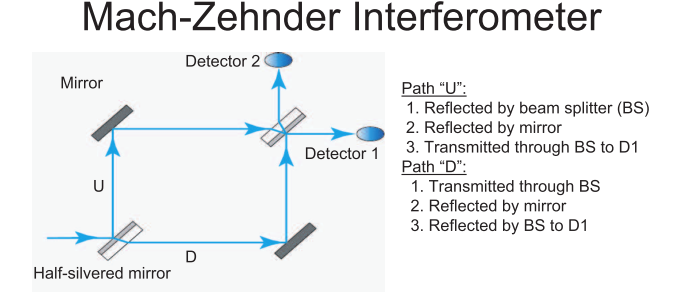
\includegraphics[scale=0.5]{Figures/mach-zender.png}
\caption{The Mach-Zehnder interferometer}
\label{mach-zehnder}
\end{figure}

As reflection results in a phase shift of $\pi$ and assuming transmission through the half-mirrors results in a phase shift of $\delta$ we easily calculate the phase differences of the two paths at the two detectors. At detector 1 and path $U$ there is a total of two reflections and a single transmission which results in a phase shift of $2\pi+\delta$. Similarly for path $D$ the phase shift is also $2\pi + \delta$. therefore at detector 1 there is constructive interference. At detector 2 path $U$ has a phase of $2\pi + 2\delta$ and path $D$ has a phase of $\pi + 2\delta$. Therefore at detector 2 there is destructive interference.\cite{dimaThesis}



\subsection{Bragg Scattering}
In neutron interferometry the crystal planes of the interferometer blades act as diffraction gratings. Incident waves that satisfy the Bragg condition \ref{bragg} are coherently scattered.
\begin{equation}
\label{bragg}
n\lambda = 2d sin(\theta_{b})
\end{equation} 
Where $n$ is a positive integer, $d$ is the distance between the atomic planes of the crystal lattice and $\theta_{b}$ is the angle between the incident beam and the atomic plane of the crystal. The amplitudes of the transmitted and the reflected beams are given by the coefficients $t$ (transmitted) and $r$ reflected.\cite{dimaThesis} 

\subsection{Quantum Scattering Theory}
\label{sec:scatteringTheory}
 Starting with the assumption the Hamiltonian has the form of 
 \begin{equation}
 \mathcal{H} = \mathcal{H}_0+\mathcal{V} \,\,\,\,\, \mathcal{H}_0= \frac{\textbf{p}^2}{2m}
 \label{eq:hamiltonian}
 \end{equation}
The presence of the potential $\mathcal{V}$ causes the solution to be different than the free particle state 
$$\mathcal{H}_0\Ket{\Phi}=E\Ket{Phi}$$

Therefore we are looking for solutions to the Schrödinger equation of the form 
\begin{equation}
\label{eq:schrodinger}
\mathcal{H}_0+\mathcal{V}\Ket{\Psi} = E\Ket{\Psi} 
\end{equation} 
 A valid solution should have that $\Ket{\Psi}\rightarrow\Ket{\Phi}$ as $\mathcal{V}\rightarrow 0$. A solution that satisfies these requirements is known as the Lippmann-Schwinger equation. 
 \begin{equation}
 	\label{lippmanSchwinger}
 	\Ket{\Psi^{\pm}}=\Ket{\Phi}+\frac{1}{E-\mathcal{H}_0\pm i\epsilon}\mathcal{V}\Ket{\Psi^{\pm}} 
 \end{equation}
 Here the energy $E$ was made slightly complex with the addition of $\pm \epsilon$ to deal with the singular nature of the operator $1/(E-\mathcal{H}_0)$. It can easily be seen that the application of the operator $E-\mathcal{H}_0$ reduces (\ref{lippmanSchwinger}) to the desired solution (\ref{eq:schrodinger}) when neglecting the imaginary component. By taking the Lipmann-Schwinger equation to the position basis explicitly it can be represented as 
 \begin{equation}
 \label{eq:positionBasis}
 \Braket{\mbox{\boldmath$x$}|\Psi^{\pm}}=\Braket{\mbox{\boldmath$x$}|\Phi} -\frac{2m}{\hbar^2} \int d^3x^{'} \frac{e^{\pm ik\left|\mbox{\boldmath$x-x^{'}$}\right|}}{ 4\pi \left| \mbox{\boldmath$x-x^{'}$} \right|} \Braket{\mbox{\boldmath$x^{'}$}|\mathcal{V}|\Psi^{\pm}}
 \end{equation}
As our scattering potentials are a function of position only the assumption can be made that the potential is \textit{local} such that it is diagonal in the position representation. Specifically the potential satisfies the requirement that 
\begin{equation}
\label{eq:localPotential}
\braket{\mbox{\boldmath$x^{'}$}|\mathcal{V}|\mbox{\boldmath$x^{''}$}}=\mathcal{V}(\mbox{\boldmath$x$}^{'})\delta^{(3)}(\mbox{\boldmath$x^{'}$}-\mbox{\boldmath$x^{''}$})
\end{equation}

Utilizing this potential we obtain 
\begin{equation}
\label{eq:localPotentialResult}
\Braket{\mbox{\boldmath$x$}|\mathcal{V}|\Psi^{\pm}}=\int d^3x^{''} \braket{\mbox{\boldmath$x^{'}$}|\mathcal{V}|\mbox{\boldmath$x^{''}$}} \braket{\mbox{\boldmath$x^{''}$}|\Psi^{\pm}}=\mathcal{V}(\mbox{\boldmath$x^{'}$})\braket{\mbox{\boldmath$x^{'}$}|\Psi^{\pm}}
\end{equation}
With this result the Lippmann-Schwinger equation can be reduced to
\begin{equation}
\label{eq:lippmannSchwingerLocal}
 \Braket{\mbox{\boldmath$x$}|\Psi^{\pm}}=\Braket{\mbox{\boldmath$x$}|\Phi} -\frac{2m}{\hbar^2} \int d^3x^{'} \frac{e^{\pm ik\left|\mbox{\boldmath$x-x^{'}$}\right|}}{ 4\pi \left| \mbox{\boldmath$x-x^{'}$} \right|} \mathcal{V}(\mbox{\boldmath$x{'}$})\Braket{\mbox{\boldmath$x^{'}$}|\Psi^{\pm}}
\end{equation}
Given that we are concerned with studying finite range scatters and that any observations that will be made will be made outside the range of the potential due to the macroscopic nature of neutron detectors the assumption can be made that $\left|\mbox{\boldmath$x$}\right| >>\left|\mbox{\boldmath$x^{'}$}\right|$. 
\begin{figure}[ht!]
\centering
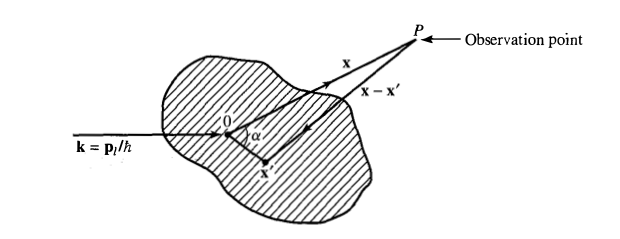
\includegraphics[scale=0.5]{Figures/scatteringObservation.png}
\caption{The finite range scattering potential. Any observations via detectors will be outside the range of the potential and therefore approximations can be made when evaluating (\ref{eq:lippmannSchwingerLocal}).}
\label{fig:finiteRangePotential}
\end{figure}

Keeping in mind this result we can define 
$$ r = \left| \mbox{\boldmath$x$} \right| $$
$$r^{'}=\left|\mbox{\boldmath$x^{'}$}\right|$$
$$\alpha = \angle(\mbox{\boldmath$x,x^{'}$})$$
$$\mbox{\boldmath$\hat{r}$} \equiv \frac{\mbox{\boldmath$x$}}{\left|\mbox{\boldmath$x$}\right|}$$

\begin{equation}
\label{eq:toObservation}
\left|\mbox{\boldmath$x-x^{'}$}\right| \approx r-\mbox{\boldmath$\hat{r}\cdot x^{'}$}
\end{equation}
\begin{equation}
\label{eq:propogationVector}
\mbox{\boldmath$k^{'}$} \equiv k\mbox{\boldmath$\hat{r}$}
\end{equation}

Utilizing equations (\ref{eq:toObservation},\ref{eq:propogationVector}) 
\begin{equation}
e^{\pm ik \left|\mbox{\boldmath$x-x^{'}$}\right|} \approx e^{\pm ikr}e^{\mp i \mbox{\boldmath$k^{'}\cdot x^{'}$}}
\label{eq:waveSimplification}
\end{equation}
For the distant $r$ at the observation point it is a useful approximation to say that 
\begin{equation}
\frac{1}{\left|\mbox{\boldmath$x-x^{'}$}\right|} \approx \frac{1}{r}
\end{equation}
Now replacing our incident generic wave with an incident plane wave $\Ket{\Phi}\rightarrow \Ket{\mbox{\boldmath$p$}}$ and using \mbox{\boldmath$k$} $\equiv \mbox{\boldmath$p_i$}/ \hbar$ To remove the $\hbar$'s from the expression. We obtain for the first term in (\ref{eq:lippmannSchwingerLocal}) 
\begin{equation}
\Braket{\mbox{\boldmath$x$}|\mbox{\boldmath$k$}}=\int d^3k^{'} \Braket{\mbox{\boldmath$x$}|\mbox{\boldmath$k^{'}$}}\Braket{\mbox{\boldmath$k^{'}$}|\mbox{\boldmath$k$}}=\int d^3k^{'}  \Braket{\mbox{\boldmath$x$}|\mbox{\boldmath$k^{'}$}} \delta^{(3)}(\mbox{\boldmath$k^{'}-k$})=\frac{e^{i\mbox{\boldmath$k \cdot x$}}}{(2\pi)^{\frac{3}{2}}}
\label{eq:PlaneWave}
\end{equation}
Using this result in (\ref{eq:lippmannSchwingerLocal}) gives an expression for the scattered wave function at a relatively distant observation point for the positive Lippmann-Schwinger wavefunction. 
\begin{equation}
\label{eq:scatteredEquation}
\Braket{\mbox{\boldmath$x$}|\Psi^{+}} = \frac{1}{(2\pi)^{\frac{3}{2}}}\left(e^{i\mbox{\boldmath$k \cdot x$}} + \frac{e^{ikr}}{r}f(\mbox{\boldmath$k^{'},k$})\right)
\end{equation}
\begin{equation}
\label{eq:f}
f(\mbox{\boldmath$k^{'},k$})=-m\left(\frac{2\pi}{h}\right)^2\Braket{\mbox{\boldmath$k^{'}$}|\mathcal{V}|\Psi^{+}}
\end{equation}
It is very easy to see that the result wavefunction is a combination of the original incident plane-wave and an outgoing spherical wave with an amplitude described by (\ref{eq:f}). An obvious issue is that here scattering has only been treated for an incident plane-wave which is not a normalizable wavefunction. In reality to describe discrete particles such as neutrons wave packet solutions are used to describe the incident particles. However, provided the size of the wave packet is much larger than the range of the finite potential $\mathcal{V}$ it is sufficient to treat an incident packet as a plane-wave.  
\subsection{Differential Cross-Section}
The scattering cross section is an important parameter for experimental scattering physics. It relates the number of particles scattering into the solid angle $d\Omega$ per unit time to the number of incident particles into an infinitesimal element $d\sigma$ of area per unit time. We search for a relation between $d\Omega$ and $d\sigma$ which we term the differential cross section given by $d\sigma/d\Omega$.
\begin{figure}[ht!]
\centering
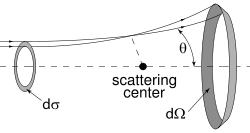
\includegraphics[scale=1.0]{Figures/scatteringCrossSection.png}
\caption{The differential cross section is the relationship between incident particles travelling through area $d\sigma$ to scattered particles crossing through the solid angle $d\Omega$}
\label{fig:scatteringCrossSection}
\end{figure}
Evidently the probability of an incident particle being within an area $d\sigma$ in time $dt$ while travelling with velocity $v$ is just 
\begin{equation}
dP = \left|\Psi_i\right|^2 dV  = \frac{1}{2\pi}^3 (vdt)d\sigma
\label{eq:incidentCross}
\end{equation}

\begin{figure}[ht!]
\centering
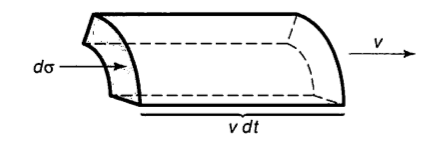
\includegraphics[scale=0.7]{Figures/incidentBeam.png}
\caption{The volume element $dV$ that a beam occupies passing through an area $d\sigma$ in time $dt$}
\label{fig:incidentBeam}
\end{figure}

Relating this probability to the probability of a particle being scattered into solid angle $d\Omega$ with equal velocity $v$ per unit time $dt$. 
\begin{equation}
\label{eq:scatteredCross}
dP=\left|\Psi_s\right|^2dV = \frac{1}{2\pi}^3 \frac{\left|f(\mbox{\boldmath$k^{'},k$})\right|^2}{r^2}(vdt)r^2 d\Omega
\end{equation}
Equations (\ref{eq:incidentCross}) and (\ref{eq:scatteredCross}) can be solved for the differential cross section 
\begin{equation}
\label{eq:differentialCrossSection}
\frac{d\sigma}{d\Omega}= \left|f(\mbox{\boldmath$k^{'},k$})\right|^2
\end{equation}

\subsection{Scattering Amplitude}
While equation (\ref{eq:f}) defines the magnitude of the outgoing spherical wave, it is defined implicitly in terms of the unknown ket $\Ket{\Psi^{+}}$. The solution to this problem in the case of sufficiently weak scatterers is to use the first Born approximation 
\begin{equation}
\label{eq:born}
\Braket{\mbox{\boldmath$x^{'}$}|\Psi^{+}} \rightarrow \Braket{\mbox{\boldmath$x^{'}$}| \Phi} = \frac{e^{i\mbox{\boldmath$x^{'}$}}}{(2\pi)^{3/2}}
\end{equation}
Combining (\ref{eq:born}) and (\ref{eq:f}) results in the first-order Born amplitude 
\begin{equation}
\label{eq:firstOrderBorn}
f^{(1)}(\mbox{\boldmath$k^{'},k$}) = -\frac{m}{2\pi\hbar^2}\int d^3x^{'}e^{i(\mbox{\boldmath$k-k^{'}$})\cdot \mbox{\boldmath$x^{'}$}}\mathcal{V}(\mbox{\boldmath$x^{'}$})
\end{equation}
As the potentials that will be dealt with are spherically symmetrical, further approximations can be made utilizing $\mbox{\boldmath$q$} \equiv \mbox{\boldmath$k-k^{'}$}$ and $$\left|\mbox{\boldmath$k-k^{'}$}\right| \equiv  q = 2ksin \left( \frac{\theta}{2}\right)$$ as seen in fig(\ref{fig:scatteringAngle}) The spherical symmetry can be used to integrate explicitly the angular component of the scattering magnitude. 
\begin{figure}[ht!]
\centering
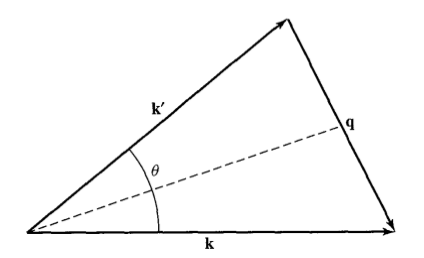
\includegraphics[scale=0.5]{Figures/scatteringAngle.png}
\caption{Scattering amplitude as a function of $\theta$ where $\mbox{\boldmath$q$}=\mbox{\boldmath$k-k^{'}$}$ }
\label{fig:scatteringAngle}
\end{figure}
$$
f^{(1)}(\theta) =  -\frac{m}{2\pi\hbar^2} \int_{r=0}^{\infty} \int_{\phi=0}^{2\pi} \int_{\theta^{'}=0}^{\pi} e^{i \left| q \right| \left| r \right|cos(\theta^{'})}sin(\theta^{'})r^2 \mathcal{V}(r) d\theta^{'} d\phi dr
$$

\begin{equation}
\label{eq:bornAngular}
= -\frac{1}{2i}\frac{2m}{\hbar^2q} \int_{0}^{\infty} r\mathcal{V}(r)(e^{iqr}-e^{-iqr})dr = -\frac{2m}{\hbar^2}\frac{1}{q}\int_{0}^{\infty} r\mathcal{V}(r)sin(qr)dr
\end{equation}
Given a potential that has spherical symmetry it is now much more simple to calculate the scattering amplitude using (\ref{eq:bornAngular}).
\subsection{Neutron-nucleus Scattering}
Generally there are two interactions that an incident neutron on a material will experience. The interaction with the nucleus of the material atoms and which is referred to as nuclear scattering and the scattering due to interaction with unpaired electrons and their magnetic moments which is known as magnetic scattering. In practice nuclear scattering is more common as it allows the structure of solids to probed. 

Given the assumptions that an incoming neutron beam will be elastically scattered and that the nucleus is fixed, the scattering will depend on the potential $V(\textbf{r})$ between the nucleus and neutron. As this is interaction is due to the strong-force it is naturally occurring over a very short range, and is approximately zero at a distance of the order $\textbf{r}=10^{-15}m$. As this is much shorter than the wavelength of thermal and cold neutrons which are used in almost all scattering experiments, the nucleus acts as a point scatterer. A neutron beam can be represented as a plane wave a wave function described by (\ref{eq:PlaneWave}) and the scattered wavefunction will take the form of (\ref{eq:scatteredEquation},\ref{eq:f}).

Due to the magnitude of the difference between the wavelength of the incident neutrons and the effective acting distance of the strong-force neutron-nucleus interaction and its approximate spherical symmetry it is an acceptable approximation to use the Fermi pseudo-potential
\begin{equation}
\label{eq:FermiPseudoPotential}
\mathcal{V}(\mbox{\boldmath$x^{'}$}) = \frac{2\pi\hbar^2}{m}b\delta(\mbox{\boldmath$x^{'}$})
\end{equation}
 as a scattering potential. Where $b$ is known as the neutron scattering length and his units of meters. For the case of multiple nuclei the potential takes the form
 \begin{equation}
 \label{eq:MultipleNuclei}
 \mathcal{V}(\mbox{\boldmath$x^{'}$})  = \frac{2\pi\hbar^2}{m}\sum\limits_{j} b_j \delta(\mbox{\boldmath$x^{'}-x_j$})
 \end{equation}

Using the spherical approximate Born solution for the amplitude (\ref{eq:firstOrderBorn}) and the Fermi pseudo-potential the scattering amplitude can be found to be 
\begin{equation}
f^{(1)}(\theta) = -\int d^3x^{'}e^{i(\mbox{\boldmath$k-k^{'}$})\cdot \mbox{\boldmath$x^{'}$}}\sum\limits_{j} b_j \delta(\mbox{\boldmath$x^{'}-x_j$})=-\sum\limits_{j}b_j e^{i(\mbox{\boldmath$q \cdot x_j$}}
\label{eq:neutronScatteringAmplitude}
\end{equation}
And in the case of a single scatterer at the origin reducing to 
\begin{equation}
f^{(1)}(\theta)  = -b
\label{eq:neutronScatteringSingle}
\end{equation}
Therefore it can be seen that the completed neutron scattered wave form is
\begin{equation}
\label{eq:scatterNeutronWaveForm}
\Braket{\mbox{\boldmath$x$}|\Psi^{+}} = \frac{1}{(2\pi)^{\frac{3}{2}}}\left(e^{i\mbox{\boldmath$k \cdot x$}} - \sum\limits_{j}b_j e^{i(\mbox{\boldmath$q \cdot x_j$}}\frac{e^{ikr}}{r}\right)
\end{equation}

From this approximate solution it is evident that the only difference between individual scatterers is their neutron scattering length $b$. The value $b$ varies greatly among even neighbouring elements in the periodic table. Unfortunately the outlined theory is not strong enough to predict the scattering length and the parameters must be determined experimentally. 

\begin{figure}[ht!]
\centering
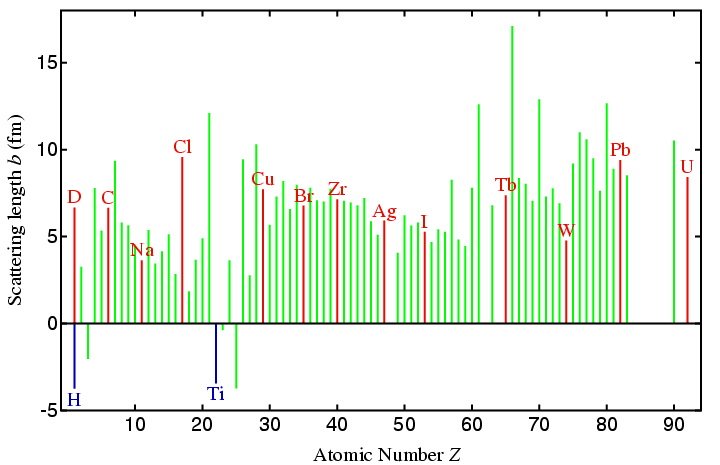
\includegraphics[scale=0.5]{Figures/neutronScatteringLength.png}
\caption{Neutron scattering lengths $b$ for the elements of the periodic table }
\label{fig:scatteringAngle}
\end{figure}

Inside a sufficiently large homogeneous material the Fermi pseudo-potential can be approximated to be 
\begin{equation}
 \mathcal{V}(\mbox{\boldmath$x^{'}$})  = \frac{2\pi\hbar^2}{m}\sum\limits_{j} b_j \delta(\mbox{\boldmath$x^{'}-x_{j}$}) \approx \frac{2\pi\hbar^2}{m}bN
 
 \label{eq:approxFermiPseudopotential}
\end{equation}
Where $N$ is the atom number density. 
\subsection{Neutron Optics}
As the neutron beam is a wavefunction many analogies from classical optics hold. The index of refraction is defined as the ratio of the speed of neutrons experiencing no potential to the speed of neutrons affected by a potential. Compared to light the form is familiar 
$$ \frac{c}{n} = \frac{K}{k}$$
Where from Schrödinger's equation
$$\Delta^2\Psi(\mbox{\boldmath$x$}) + \frac{2m}{\hbar^2}(E-\mathcal{V}(\mbox{\boldmath$x$})\Psi(r) = 0 $$ 
\begin{equation}
\label{eq:K}
K^2 = \frac{2m}{\hbar^2}(E-\mathcal{V}(\mbox{\boldmath$x$}))
\end{equation}
\begin{equation}
\label{eq:nofr}
n(\mbox{\boldmath$x$}) = \frac{K}{k} = \sqrt{\frac{E-\mathcal{V}(\mbox{\boldmath$x$})}{E}=\sqrt{1-\frac{\mathcal{V}(\mbox{\boldmath$x$})}{E}}
\end{equation}
Given that the neutron scattering potentials are described by (\ref{eq:approxFermiPseudopotential}) the index of refraction can be approximated to 
\begin{equation}
V(\mbox{\boldmath$x$}) = \sqrt{1-\frac{\frac{2\pi\hbar^2}{m}bN}{E}}
\label{eq:indexofrefraction}
\end{equation}

In the case of magnetic materials the magnetic potential
$$\mathcal{V_{mag}(\mbox{\boldmath$x$})=-\mbox{\boldmath$u\cdot B_{eff}$}$$ must be accounted for. This results in an index of refracton for magnetic materials such as Fe,Ni and Co of 
\begin{equation}
n_{\pm}(\mbox{\boldmath$x$})= \sqrt{1-\frac{\frac{2\pi\hbar^2}{m}bN \mp \mbox{\boldmath$u\cdot B_{eff}$}}{E}}
\label{eq:nucleurIndexofRefraction}
\end{equation}
\subsection{Neutron Wave Guides}

